% ========================================
% CAPSTONE I - UDLA (entrega final: informe de avance)
% Basado en template_capstone_clase.tex (Christian Pieringer, v2.0), clase udla-capstone
% Compilar:  latexmk -pdf capstone_report_ef.tex     (requiere biber)
% ========================================

\documentclass{udla-capstone}

\proyectotitulo{Auditoría y prevención de fuga de datos en pipelines de Machine Learning generados por LLM}
\proyectoautor{Witman Zavala Muñoz}
\proyectoprofesor{Francisco Pérez}
\proyectocoprofesor{No aplica}
\proyectofecha{Octubre, 2026}
\proyectociudad{Santiago de Chile}

\addbibresource{references.bib}
% Todas las fuentes están en inglés: APA 7 pone sus títulos en tipo oración
\DeclareSourcemap{\maps[datatype=bibtex]{\map{\step[fieldset=langid, fieldvalue=english]}}}
% APA 7: rangos de páginas con raya corta
\DefineBibliographyExtras{english}{\protected\def\bibrangedash{\textendash\penalty\hyphenpenalty}}
\DefineBibliographyExtras{spanish}{\protected\def\bibrangedash{\textendash\penalty\hyphenpenalty}}

% Las figuras se leen directamente de la carpeta de resultados: así nunca quedan desactualizadas.
\graphicspath{{../../04_experiments/results/}}

% Notación y ayudas
\newcommand{\DOpt}{\ensuremath{\Delta\mathrm{Opt}}}
\newcommand{\arch}[1]{\texttt{\detokenize{#1}}}   % nombres de archivo con guiones bajos
\newcommand{\nota}[1]{\par\noindent{\footnotesize\textit{Nota.} #1}\par\smallskip}
\newcommand{\donde}[1]{\par\noindent{\footnotesize\textbf{Donde:} #1}\par\smallskip}
\setlength{\tabcolsep}{4pt}

\begin{document}

\pagenumbering{roman}

\portada

\newpage

\begin{resumen}
Los asistentes de programación basados en modelos de lenguaje grande (LLM) ya escriben pipelines de Machine Learning completos. Entre sus posibles errores, la fuga de datos es el único que no interrumpe la ejecución e infla las métricas de evaluación: un transformador (escalador, imputador, selector de variables) que se ajusta con todas las filas antes de separar entrenamiento y prueba produce un modelo que parece mejor de lo que es. Este informe presenta un auditor determinista que combina el análisis del árbol sintáctico (AST) con la verificación en ejecución, un refactorizador que repara los patrones habituales sin cambiar el modelo y un indicador de Sesgo de Optimismo (\DOpt) que mide cuánto infla la fuga una métrica. Se evaluó sobre 96 pares de scripts con y sin fuga (6 datasets de scikit-learn, 4 familias de algoritmos y 4 tipos de fuga) y sobre 13 scripts escritos a mano como prueba independiente. El auditor acierta el 100\,\% del banco de control, que es una evaluación circular; en la prueba independiente el AST detecta 8 de 9 casos con fuga, la ejecución 7 de 9 y la combinación 9 de 9. El optimismo medido es casi nulo en clasificación (efecto techo) y de hasta 0,07 de $R^2$ en regresión; con señal nula la selección con fuga infla el AUC hasta 0,20. Los productos son dos Agent Skills y una plataforma web. Aún no se han generado pipelines con LLM reales; esa medición es el objetivo de Capstone~II.

\medskip
\noindent\textbf{Para un público no técnico.} Cuando una IA escribe un programa que aprende de datos, puede cometer un error silencioso: «espiar» las respuestas de la evaluación final mientras aprende, de modo que el resultado parece mejor de lo real. Este proyecto construye un revisor automático que encuentra ese error, lo corrige y calcula cuánto exageraba el resultado.
\end{resumen}
\addcontentsline{toc}{section}{Resumen}

\begin{center}
    \textbf{Palabras clave:} fuga de datos; LLM; auditoría de código; scikit-learn; análisis estático; sesgo de optimismo.
\end{center}

\newpage

\begin{abstract}
LLM-based coding assistants already write end-to-end Machine Learning pipelines. Among their possible errors, data leakage is the only one that neither interrupts execution nor leaves evidence in the code, and it inflates evaluation metrics. This report presents a deterministic auditor that combines abstract syntax tree (AST) analysis with runtime verification, a refactoring tool that repairs common patterns without changing the model, and an Optimism Bias indicator (\DOpt) that measures how much leakage inflates a metric. It was evaluated on 96 pairs of leaky and clean scripts (6 scikit-learn datasets, 4 algorithm families, 4 leakage types) and on 13 hand-written scripts as an independent test. The auditor scores 100\,\% on the control bank, which is a circular evaluation; on the independent test the AST detects 8 of 9 leaky cases, runtime verification 7 of 9, and their combination 9 of 9. Measured optimism is almost null in classification (ceiling effect) and up to 0.07 of $R^2$ in regression; with null signal, leaky feature selection inflates AUC by up to 0.20. The products are two Agent Skills and a web platform. No pipelines from real LLMs have been generated yet; that measurement is the goal of Capstone II.
\end{abstract}
\addcontentsline{toc}{section}{Abstract}

\begin{center}
    \textbf{Keywords:} data leakage; LLM; code auditing; scikit-learn; static analysis; optimism bias.
\end{center}

\newpage

\tableofcontents

\newpage

\pagenumbering{arabic}

% ========================================
% CAPÍTULO 1: INTRODUCCIÓN Y FORMULACIÓN DEL PROBLEMA  (criterio 1 de la rúbrica)
% ========================================

\chapter{INTRODUCCIÓN Y FORMULACIÓN DEL PROBLEMA}
\label{ch:introduccion}

\section{Contexto}

Los asistentes de programación basados en modelos de lenguaje grande (LLM) ya escriben pipelines completos de ciencia de datos \parencite{hong2025} y se evalúan con \emph{benchmarks} de generación de código \parencite{lai2023}, y los \emph{benchmarks} de agentes miden su puntaje o su tasa de éxito \parencite{chan2025,huang2024}, no la validez metodológica de lo que producen. Un código generado por un LLM puede fallar de siete formas habituales: (1) errores de sintaxis; (2) alucinación de APIs o uso de métodos obsoletos; (3) incompatibilidad de dimensiones o tipos; (4) ineficiencia o agotamiento de memoria; (5) falta de control de semillas; (6) manejo inseguro de archivos o credenciales; y (7) \textbf{fuga de datos} (\emph{data leakage}).

La fuga es el único de los siete que \textbf{no interrumpe la ejecución}. Los fallos 1 a 4 y 6 producen una excepción o son visibles para un \emph{linter}, y el fallo 5 se detecta repitiendo la corrida. En cambio, la fuga produce un script que corre de principio a fin, entrega métricas más altas y, por eso, rara vez se cuestiona (Tabla~\ref{tab:ruidoso}). En la práctica humana el problema es amplio: \textcite{kapoor2023} hallaron 294 artículos afectados por fuga en 17 campos científicos, y \textcite{kaufman2012} la formularon como información del objetivo que no estaría disponible al predecir.

\begin{table}[!htbp]
\centering
\caption{Fallos ruidosos frente a fallo silencioso en código de ML generado por LLM.}
\label{tab:ruidoso}
\begingroup\footnotesize\singlespacing
\begin{tabular}{@{}p{3.4cm} p{4.6cm} p{7.4cm}@{}}
\toprule
Dimensión & Fallos ruidosos (1--4 y 6) & Fuga de datos (7) \\
\midrule
Comportamiento del intérprete & Lanza una excepción & Se ejecuta sin error ni advertencia \\
Detección estándar & Intérprete o \emph{linter} & Invisible para herramientas convencionales: tipos y dimensiones coinciden \\
Efecto sobre las métricas & No llega a producirlas & Las infla (optimismo) \\
Riesgo en producción & Bajo: el pipeline no corre & Alto: el modelo se despliega con una capacidad de generalización peor que la creída \\
\bottomrule
\end{tabular}
\endgroup
\end{table}

\section{Qué es la fuga y cómo ocurre en scikit-learn}

Un transformador (escalador, imputador, selector de variables, PCA) \emph{aprende} parámetros con \texttt{.fit()}: medias y desviaciones, vecinos más cercanos, o qué variables conservar. Si aprende con \textbf{todas} las filas antes de separar entrenamiento y prueba, o fuera de un \texttt{Pipeline} dentro de una validación cruzada, ya vio las filas que luego se usan para evaluar. Formalmente, el aislamiento correcto exige que los parámetros del preprocesamiento sean función solo de los datos de entrenamiento; hay fuga cuando algún parámetro se estima con la unión de entrenamiento y prueba. La Figura~\ref{fig:codigo} contrasta ambas formas con el mismo modelo, los mismos datos y los mismos pliegues.

\begin{figure}[!htbp]
\centering
\begin{footnotesize}
\begin{verbatim}
# CON FUGA: el escalador ve todas las filas
X_esc = StandardScaler().fit_transform(X)
scores = cross_val_score(modelo, X_esc, y, cv=5)

# SIN FUGA: en cada pliegue, .fit() ve solo el entrenamiento
pipe = Pipeline([("escalador", StandardScaler()), ("modelo", modelo)])
scores = cross_val_score(pipe, X, y, cv=5)
\end{verbatim}
\end{footnotesize}
\caption{Misma operación con y sin fuga de datos.}
\label{fig:codigo}
\end{figure}

Para ver el mecanismo con números, el script \arch{leakage_demo.py} ejecuta ambas formas con \texttt{breast\_cancer}, un \texttt{KNNImputer}, un escalador, \texttt{SelectKBest} y una red \texttt{MLPClassifier}, con los mismos pliegues (Figura~\ref{fig:demo}). Con datos reales, el ROC-AUC es 0,979 con fuga y 0,977 sin ella: $\DOpt=+0{,}0015$, casi invisible porque la señal es muy fuerte. Con 500 columnas de ruido y etiquetas permutadas (verdad: AUC $=0{,}5$), sube a 0,571 frente a 0,523 ($\DOpt=+0{,}048$): el selector «encuentra» columnas que por azar parecen predecir.

\begin{figure}[!htbp]
\centering
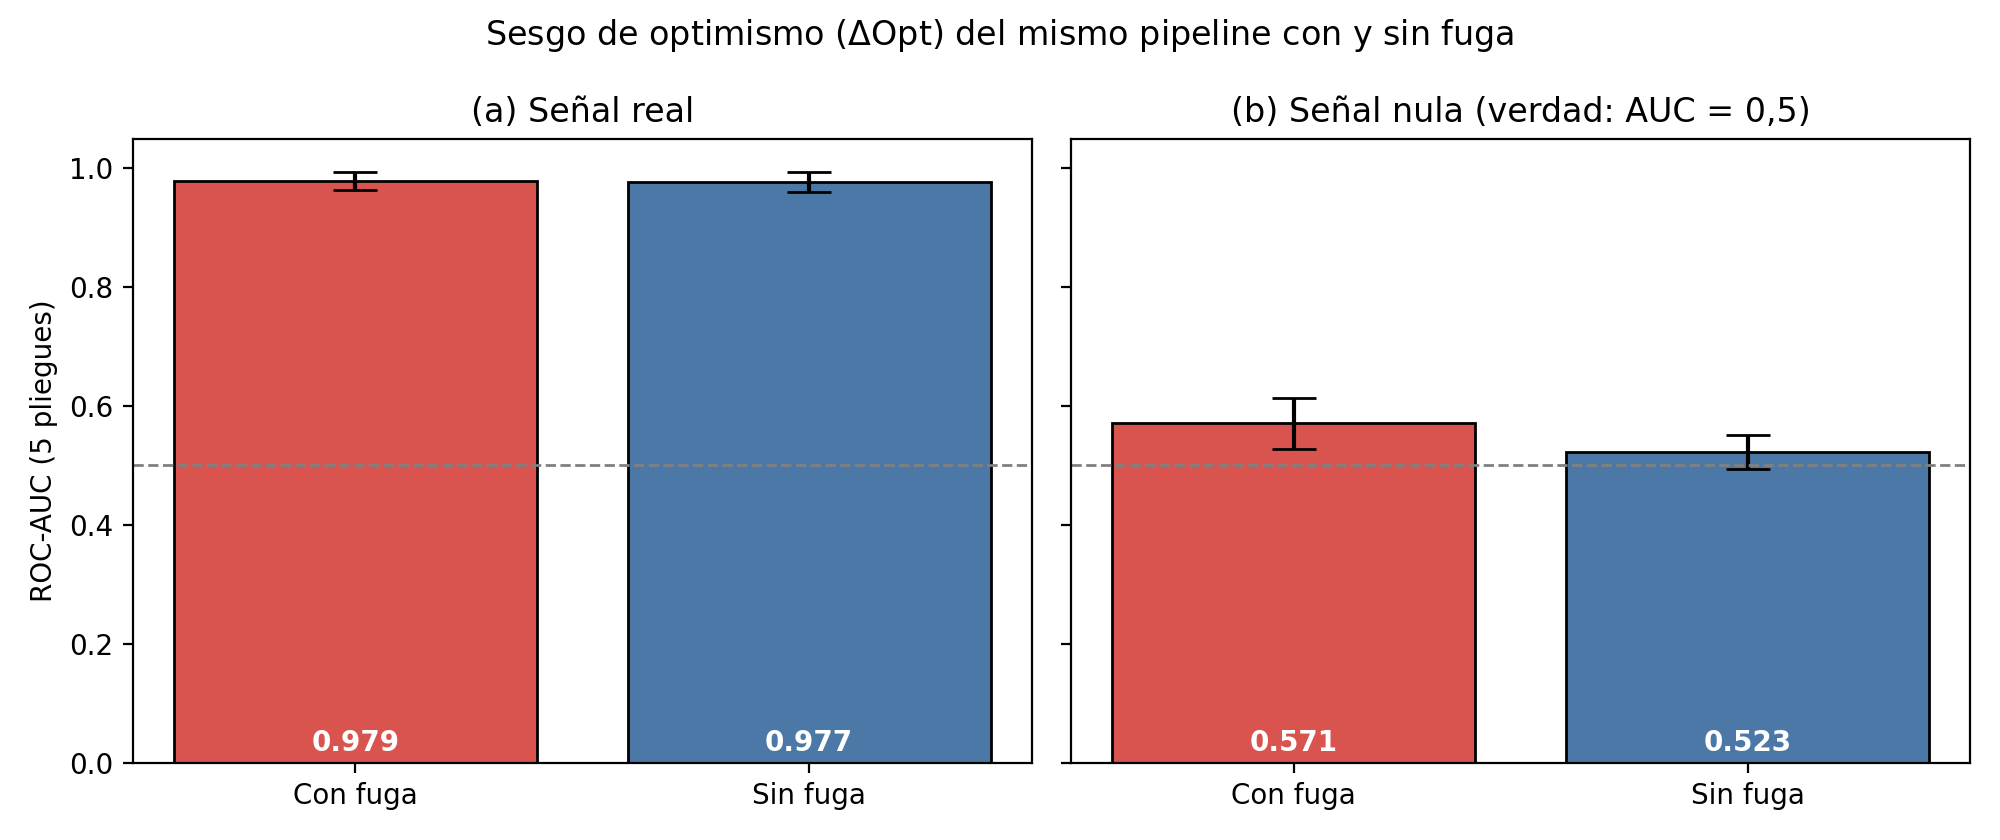
\includegraphics[width=0.72\textwidth]{fig_leakage_demo.png}
\caption{Mismo pipeline con y sin fuga. (a) Señal real. (b) Señal nula; la línea punteada marca el AUC verdadero (0,5).}
\label{fig:demo}
\end{figure}

Se estudian cuatro mecanismos: \textbf{escalado} (la media y la varianza incluyen filas de prueba), \textbf{imputación} (\texttt{KNNImputer} puede copiar valores de vecinos de prueba), \textbf{selección de variables} (\texttt{SelectKBest} usa las etiquetas de todas las filas) y \textbf{combinada} (los tres a la vez).

\section{Problema, pregunta y relevancia}

\textbf{Problema.} Un script de ML tabular puede contener fuga de datos sin que nada lo advierta, y quien recibe ese código de un asistente de IA no tiene una forma barata de comprobarlo ni de saber cuánto distorsiona la evaluación.

\textbf{Pregunta de investigación.} ¿Es posible detectar automáticamente, leyendo y ejecutando el código, la fuga de preprocesamiento y selección en pipelines de scikit-learn; reparar el código sin cambiar el modelo; y cuantificar cuánto optimismo introduce la fuga en distintas familias de algoritmos?

\textbf{Relevancia.} Los detectores existentes son principalmente estáticos y se evaluaron sobre código humano \parencite{yang2022,drobnjakovic2024,alomar2025}, y los LLM tienen dificultades para identificar por sí mismos estos problemas tempranos del pipeline \parencite{kumar2025}. Falta un instrumento determinista que audite código de asistentes, lo repare y mida el daño; ese es el entregable de este proyecto.

\section{Objetivos}

\textbf{Objetivo general.} Diseñar, validar empíricamente e implementar un marco automatizado de detección y prevención de fuga de datos en pipelines de aprendizaje supervisado con scikit-learn, y cuantificar el sesgo de optimismo que induce en cuatro familias de algoritmos.

\begin{table}[!htbp]
\centering
\caption{Objetivos específicos verificables y evidencia.}
\label{tab:oe}
\begingroup\footnotesize\singlespacing
\begin{tabular}{@{}l p{9.4cm} p{4.4cm}@{}}
\toprule
OE & Objetivo específico & Evidencia \\
\midrule
OE1 & Formalizar los mecanismos de fuga (escalado, imputación, selección, combinada) y distinguirlos de otros fallos de código generado. & Secciones 1.1--1.2; banco de 96 pares \\
OE2 & Desarrollar un auditor determinista (AST y verificación en ejecución) y medir su precisión, recall y VPN contra una verdad conocida. & Tablas~\ref{tab:banco} y \ref{tab:indep} \\
OE3 & Cuantificar el Sesgo de Optimismo \DOpt{} por tipo de fuga y familia (RandomForest, Gradient Boosting, lineal regularizado y red neuronal MLP) en 3 datasets de clasificación y 3 de regresión. & Tablas~\ref{tab:dopt} y \ref{tab:tests}; Figuras~\ref{fig:heatmap} y \ref{fig:ruido} \\
OE4 & Entregar dos Agent Skills y una plataforma web que permitan auditar, reparar y crear pipelines sin fuga. & Capítulo~\ref{ch:aplicabilidad} \\
\bottomrule
\end{tabular}
\endgroup
\end{table}

\section{Métrica central y criterios de éxito}

La métrica es el \textbf{Sesgo de Optimismo Inducido por Fuga}:
\begin{equation}
\DOpt = M_{\mathrm{leaky}} - M_{\mathrm{clean}},
\end{equation}
donde $M$ es el promedio de una métrica (ROC-AUC, F1, $R^2$ o $-$RMSE) en 5 pliegues, y $M_{\mathrm{leaky}}$ y $M_{\mathrm{clean}}$ provienen del mismo dataset, los mismos pliegues (semilla 42), el mismo modelo y los mismos hiperparámetros: solo cambia si el preprocesamiento se ajustó con todas las filas o dentro de un \texttt{Pipeline}. Por construcción, si no hay fuga, $\DOpt=0$. La sección~\ref{sec:alternativas} justifica por qué se descarta la «brecha de generalización», que mide sobreajuste y no fuga.
\donde{$\DOpt$: sesgo de optimismo; $M_{\mathrm{leaky}}$: métrica promedio del pipeline con fuga; $M_{\mathrm{clean}}$: métrica promedio del mismo pipeline sin fuga (preprocesamiento dentro de un \texttt{Pipeline}); un valor positivo indica que la fuga mejora artificialmente la métrica.}

\begin{table}[!htbp]
\centering
\caption{Criterios de éxito operativos y resultado (detalle en los capítulos~\ref{ch:validacion} y \ref{ch:interpretacion}).}
\label{tab:exito}
\begingroup\footnotesize\singlespacing
\begin{tabular}{@{}l p{7.6cm} p{6.4cm}@{}}
\toprule
OE & Criterio (umbral o punto de comparación) & Resultado \\
\midrule
OE2 & Banco de control: precisión y recall $\geq 0{,}90$ & 1,00 y 1,00 (evaluación \textbf{circular}, ver sección~\ref{sec:eficacia}) \\
OE2 & Evaluación independiente (13 scripts manuales): recall híbrido $\geq 0{,}80$ y 0 falsos positivos & 9/9 y 0 FP; IC95\,\% exacto del recall [0,66; 1,00]: \textbf{con $n=9$ no se puede afirmar} el umbral \\
OE3 & H-esc.: en árboles, \DOpt{} por escalado $\approx 0$ ($|\DOpt|<0{,}001$) & Confirmada: máximo 0,0002 \\
OE3 & H-MLP: la red neuronal sufre el mayor \DOpt & \textbf{Parcial}: solo en regresión y sin significancia tras corregir por multiplicidad \\
OE4 & Reparación automática $\geq 90$\,\% de los scripts con fuga & 96/96 en el banco; \textbf{4/9} en la evaluación independiente \\
\bottomrule
\end{tabular}
\endgroup
\end{table}
\nota{H-esc.: hipótesis del escalado en árboles; H-MLP: hipótesis de mayor vulnerabilidad de la red neuronal; FP: falsos positivos. Los umbrales son propuestas del autor, formalizadas después de la prueba piloto descrita aquí; en Capstone~II se fijarán antes de evaluar con pipelines de LLM reales.}

\section{Alcance, supuestos y restricciones}

\emph{Alcance:} clasificación y regresión supervisadas con scikit-learn sobre datos tabulares; fuga de preprocesamiento, imputación y selección de variables. El \emph{clustering} queda fuera porque no hay un objetivo explícito contra el cual medir el optimismo. \emph{Supuestos:} datos i.i.d.; 5 pliegues con semilla fija; el generador de pares reproduce con fidelidad el mecanismo de fuga. \emph{Restricciones:} solo datasets nativos de scikit-learn y sin anotadores humanos (observaciones del comité); no se auditan fugas temporales ni de dominio; los pipelines escritos por LLM reales \textbf{aún no se han generado} (Capstone~II).

\section{Retroalimentación de la primera entrega: matriz de trazabilidad}
\label{sec:retro}

Las observaciones del comité apuntan a validar primero los cimientos (problema, métrica, datos y protocolo) y a eliminar la variabilidad no controlada, como los anotadores humanos. La Tabla~\ref{tab:retro} vincula cada una con su diagnóstico, la solución y la sección donde se verifica. En la forma, toda figura y tabla tiene \emph{caption} numerado y se cita en el texto, y cada cifra proviene de los archivos de resultados del repositorio.

\begin{table}[!htbp]
\centering
\caption{Matriz de trazabilidad entre las observaciones del comité y su resolución.}
\label{tab:retro}
\begingroup\scriptsize\singlespacing
\begin{tabular}{@{}l p{3.3cm} p{3.6cm} p{5.6cm} p{1.9cm}@{}}
\toprule
Cód. & Requerimiento del comité & Diagnóstico & Solución adoptada & Dónde \\
\midrule
R1 & Contextualizar los fallos de los LLM y justificar por qué estudiar solo la fuga & La elección parecía arbitraria, sin una taxonomía de defectos & Distinción entre fallos ruidosos (\emph{fail-stop}) y el fallo silencioso de la fuga, único que no detiene la ejecución e infla la métrica & Sec.~1.1, Tabla~\ref{tab:ruidoso} \\
R2 & Especificar qué modelos generan y cuáles auditan & Riesgo de sesgo de autoconfirmación si un LLM se evalúa a sí mismo & Separación estricta: LLM generadores como sujetos de estudio; auditor determinista (AST y ejecución) que nunca consulta a un LLM & Sec.~\ref{sec:arquitectura}, Tabla~\ref{tab:arquitectura} \\
R3 & Mostrar cómo se fugan los datos con un ejemplo simple & La formulación abstracta impedía ver el mecanismo & Ejemplo de código con y sin fuga y script comentado paso a paso que genera un gráfico comparativo & Sec.~1.2, Figuras~\ref{fig:codigo} y~\ref{fig:demo} \\
R4 & Explicar el experimento en la práctica, paso a paso & El flujo anterior de 19 etapas era difícil de auditar & Protocolo lineal de cinco fases deterministas, cada una con un script y un artefacto verificable & Sec.~\ref{sec:fases}, Tabla~\ref{tab:etapas} \\
R5 & Usar datasets de scikit-learn y evitar anotadores humanos & Datos externos y etiquetado manual agregan variabilidad subjetiva & Seis datasets nativos de \texttt{sklearn.datasets}; verdad conocida por construcción (oráculo programático) & Sec.~\ref{sec:datos} y~\ref{sec:fases} \\
R6 & Elegir el paradigma y las familias de modelos & Faltaba acotar la tarea y justificar la sensibilidad de cada familia & Clasificación y regresión supervisadas; cuatro familias (árboles, \emph{boosting}, lineal regularizado y MLP) con hipótesis explícitas & Sec.~1.5--1.6 \\
R7 & Dejar todo en GitHub y poder explicar el código & Se requería trazabilidad computacional y dominio técnico & Repositorio público modular, un comando de reproducción y scripts comentados por bloques & Anexo~\ref{an:repro} \\
R8 & Definir como producto una o varias \emph{Skills} & Faltaba un entregable transferible & Dos Agent Skills y una plataforma web en Streamlit como alternativa gráfica & Cap.~\ref{ch:aplicabilidad} \\
R9 & Validar la métrica («brecha de generalización auditada») & El nombre se confundía con el sobreajuste & Sesgo de Optimismo Inducido por Fuga, \DOpt, medido con pliegues idénticos & Sec.~1.5 \\
\bottomrule
\end{tabular}
\endgroup
\end{table}

% ========================================
% CAPÍTULO 2: FUNDAMENTACIÓN Y POSICIONAMIENTO  (criterio 2)
% ========================================

\chapter{FUNDAMENTACIÓN Y POSICIONAMIENTO}
\label{ch:fundamentacion}

El proyecto exige tres decisiones que la literatura permite justificar: cómo \emph{detectar} la fuga, cómo \emph{medir} su efecto y contra qué \emph{verdad de referencia} validar el detector. Este capítulo compara las alternativas para cada una y deriva de esa comparación la brecha y las decisiones de diseño.

\section{La fuga como sesgo de evaluación}

\textcite{kaufman2012} definen la fuga como el uso, durante el entrenamiento o la evaluación, de información que no estaría disponible al momento de predecir. En preprocesamiento, el caso más estudiado es la selección de variables: \textcite{ambroise2002} mostraron que elegir genes con todas las muestras y validar después produce tasas de error engañosamente bajas, y \textcite{varma2006} y \textcite{cawley2010} demostraron que optimizar decisiones con los mismos datos con que se estima el desempeño sesga esa estimación hacia el optimismo. \textcite{hastie2009} lo resumen como la forma «incorrecta» y la «correcta» de validar: todo paso que mira los datos debe repetirse dentro de cada pliegue. La amplitud del problema en la práctica es conocida: \textcite{kapoor2023} documentaron 294 artículos afectados en 17 campos. Esta literatura sustenta dos hipótesis del proyecto: la selección supervisada debería ser la fuga más dañina cuando la señal es débil, y un transformador afín, como el escalado, no debería afectar a los árboles.

\section{Alternativas para detectar la fuga}

La Tabla~\ref{tab:enfoques} compara cuatro enfoques. Los \textbf{detectores estáticos} analizan el flujo de datos de notebooks \parencite{yang2022}, lo formalizan con interpretación abstracta \parencite{drobnjakovic2024} o lo integran a un IDE \parencite{alomar2025}. Los \textbf{LLM como detector} combinan \emph{slicing} con \emph{prompts} estructurados \parencite{draoui2026} o integran un agente de chequeo de fuga \parencite{nam2025}, pero como jueces prefieren sus propias respuestas \parencite{zheng2023} y fallan al identificar problemas tempranos del pipeline \parencite{kumar2025}. Las \textbf{listas de verificación} \parencite{lones2024,kapoor2024} dependen de un revisor experto. La \textbf{instrumentación en ejecución} observa con cuántas filas se ajustó cada transformador, a costa de ejecutar el código.

\begin{table}[!htbp]
\centering
\caption{Síntesis comparativa de los enfoques para detectar fuga de datos.}
\label{tab:enfoques}
\begingroup\scriptsize\singlespacing
\begin{tabular}{@{}p{2.6cm} p{3.6cm} p{4.3cm} p{1.6cm} p{2.6cm}@{}}
\toprule
Enfoque & Fortaleza & Limitación & ¿Mide el daño? & Uso en este proyecto \\
\midrule
Análisis estático (flujo de datos) & Determinista, reproducible, no ejecuta código & Ciego a fugas que dependen de valores y a alias; validado en código humano & No & Núcleo del auditor (AST) \\
LLM como detector o juez & Entiende estilos variados de código & Sesgo de autopreferencia, variabilidad entre corridas, sin evidencia trazable & No & Descartado como instrumento \\
Listas de verificación & Cubren fugas temporales y de dominio & Requieren un revisor experto; no se automatizan & No & Criterio de «código correcto» \\
Instrumentación en ejecución & Observa el ajuste real, inmune a alias & Exige ejecutar código no confiable & No & Segunda opinión del auditor \\
\textbf{Este proyecto (híbrido)} & Lee y ejecuta; repara patrones comunes & Solo scikit-learn tabular; reparación limitada & \textbf{Sí} (\DOpt) & --- \\
\bottomrule
\end{tabular}
\endgroup
\end{table}

\section{Alternativas para medir el efecto y para la verdad de referencia}
\label{sec:alternativas}

Para \textbf{medir el daño}, la \emph{brecha de generalización} (entrenamiento menos prueba) mide sobreajuste, que existe aun sin fuga (por ejemplo, en un árbol sin poda), y confunde dos fenómenos. La \emph{validación cruzada anidada} corrige el sesgo de selección de modelos \parencite{varma2006,cawley2010}, pero no aísla el aporte de un error concreto del código. La \emph{comparación pareada} de una evaluación defectuosa con su versión corregida, con los mismos pliegues, sí lo aísla, porque todo lo demás queda fijo; es la lógica de los reanálisis de \textcite{kapoor2023} y la que adopta \DOpt.

Para la \textbf{verdad de referencia}, los anotadores humanos introducen variabilidad subjetiva y el LLM juez hereda los problemas de la Tabla~\ref{tab:enfoques}. El oráculo programático, que construye cada script con y sin fuga, conoce la etiqueta con certeza, pero si el mismo autor escribe el generador y el detector la evaluación es circular; por eso se complementa con un conjunto escrito a mano con estilos que el generador no produce.

\section{Brecha y decisiones de diseño}

Entre las fuentes revisadas, ninguna mide el optimismo mediante una intervención pareada sobre el mismo pipeline ni combina la lectura y la ejecución del código con su reparación. La Tabla~\ref{tab:decisiones} resume las decisiones que se derivan de la comparación anterior.

\begin{table}[!htbp]
\centering
\caption{Decisiones de diseño, alternativas descartadas y respaldo.}
\label{tab:decisiones}
\begingroup\scriptsize\singlespacing
\begin{tabular}{@{}p{3.0cm} p{3.4cm} p{6.0cm} p{2.4cm}@{}}
\toprule
Decisión & Alternativa descartada & Justificación & Respaldo \\
\midrule
Auditor determinista (AST y ejecución) & LLM como juez & Un instrumento de medición debe dar el mismo veredicto en cada corrida y no puede tener interés en el resultado & \textcite{zheng2023} \\
Detector híbrido & Solo estático o solo dinámico & El AST no ve valores ni alias; la ejecución no ve ajustes parciales: fallan en casos distintos & \textcite{yang2022} \\
\DOpt{} pareado (mismos pliegues) & Brecha de generalización; CV anidada & Aísla causalmente el efecto del error; la brecha mezcla fuga y sobreajuste & \textcite{kapoor2023,cawley2010} \\
Oráculo programático más un conjunto manual independiente & Anotadores humanos o LLM juez & Etiqueta exacta y sin subjetividad; el conjunto manual controla la circularidad & \textcite{hevner2004} \\
Columnas de ruido y control positivo con señal nula & Solo datos originales & La fuga por selección solo se manifiesta si hay variables inútiles entre las cuales elegir & \textcite{ambroise2002} \\
Pruebas no paramétricas pareadas con corrección de Holm & $t$ de Student sin corregir & Pocos datasets y sin supuesto de normalidad; varias pruebas simultáneas & \textcite{demsar2006,holm1979} \\
\bottomrule
\end{tabular}
\endgroup
\end{table}

% ========================================
% CAPÍTULO 3: METODOLOGÍA, DATOS Y HOJA DE RUTA  (criterio 3)
% ========================================

\chapter{METODOLOGÍA, DATOS Y HOJA DE RUTA}
\label{ch:metodologia}

\section{Metodología: protocolo experimental en cinco fases}
\label{sec:fases}

Se adapta CRISP-DM a la construcción de un instrumento de medición: siguiendo la lógica de \emph{design science}, se construye un artefacto y se evalúa contra una verdad conocida \parencite{hevner2004}. El flujo anterior, de 19 etapas, se reemplazó por un protocolo lineal de cinco fases deterministas (Tabla~\ref{tab:etapas}). Cada fase tiene un propósito ligado a un objetivo específico, un script que la ejecuta y un artefacto que la deja verificable; todas se reproducen con \arch{python run_all.py}.

\begin{table}[!htbp]
\centering
\caption{Protocolo en cinco fases: propósito, implementación y evidencia.}
\label{tab:etapas}
\begingroup\scriptsize\singlespacing
\begin{tabular}{@{}p{2.7cm} p{2.0cm} p{3.9cm} p{3.4cm} p{2.3cm} p{0.8cm}@{}}
\toprule
Fase & CRISP-DM & Propósito & Script & Artefacto & OE \\
\midrule
0. Datos & Comprensión y preparación & Cargar y caracterizar 6 datasets; ruido y faltantes reproducibles & \arch{sklearn_loader.py}; \arch{eda_datasets.py} & \arch{eda_datasets.csv} & OE3 \\
1. Banco de control & Preparación & Escribir 96 pares con y sin fuga (oráculo programático) & \arch{generate_controlled_pairs.py} & 192 scripts & OE1 \\
2. Auditoría & Modelado del instrumento & Auditar cada script con AST y con verificación en ejecución & \arch{03_auditor/}; \arch{run_benchmark.py} & \arch{auditor_per_script.csv} & OE2 \\
3. Eficacia del auditor & Evaluación & Comparar veredictos con la verdad conocida y con la línea base & \arch{run_benchmark.py}; \arch{independent_evaluation.py} & Tablas \ref{tab:banco}--\ref{tab:base} & OE2 \\
4. Sesgo de optimismo & Evaluación & Calcular \DOpt{} por par, pruebas por familia y control positivo & \arch{statistical_analysis.py}; \arch{noise_sensitivity.py} & Tablas \ref{tab:dopt}--\ref{tab:tests} & OE3 \\
5. Empaquetado & Despliegue & Publicar el auditor como dos Skills y una plataforma web & \arch{05_skills/}; \arch{06_web_app/} & Cap.~\ref{ch:aplicabilidad} & OE4 \\
\bottomrule
\end{tabular}
\endgroup
\end{table}
\donde{OE: objetivo específico. La fase 0 prepara los insumos de las cinco fases experimentales.}

\section{Datos: origen, obtención y caracterización}
\label{sec:datos}

Se usan seis conjuntos nativos de scikit-learn (Tabla~\ref{tab:datasets}): tres de clasificación (\texttt{breast\_cancer}, \texttt{wine}, \texttt{digits}) y tres de regresión (\texttt{diabetes}, \texttt{california\_housing}, \texttt{make\_friedman1}). Son públicos, no contienen datos personales y se cargan sin copiarlos al repositorio; solo \texttt{california\_housing} se descarga la primera vez. La Figura~\ref{fig:eda} resume la dispersión de escalas y el balance de clases.

\begin{table}[!htbp]
\centering
\caption{Caracterización de los datasets.}
\label{tab:datasets}
\begingroup\footnotesize\singlespacing
\begin{tabular}{@{}l l l r r r r r@{}}
\toprule
ID & Dataset & Tarea & $N$ & Variables & Razón de escalas & Asimetría media & Clase minoritaria \\
\midrule
D1 & breast\_cancer & Clasif. (2) & 569 & 30 & 215.171 & 1,74 & 37,3\,\% \\
D2 & wine & Clasif. (3) & 178 & 13 & 2.530 & 0,43 & 27,0\,\% \\
D3 & digits & Clasif. (10) & 1.797 & 64 & 277 & 4,89 & 9,7\,\% \\
D4 & diabetes & Regresión & 442 & 10 & 1,0 & 0,41 & --- \\
D5 & california\_housing & Regresión & 3.000$^{*}$ & 8 & 1.398 & 10,00 & --- \\
D6 & friedman1 & Regresión & 1.000 & 50 & 1,1 & 0,04 & --- \\
\bottomrule
\end{tabular}
\endgroup
\end{table}
\nota{Razón de escalas: desviación estándar máxima sobre mínima entre variables. $^{*}$Submuestra determinista de 3.000 filas de 20.640 (desviación B1, sección~\ref{sec:desviaciones}). \texttt{digits} tiene 3 columnas constantes.}

\textbf{Calidad más allá de los faltantes.} Ningún dataset base tiene filas duplicadas. La proporción de celdas atípicas ($|z|>3$ por columna) es baja: 1,24\,\% en \texttt{breast\_cancer}, 0,48\,\% en \texttt{wine}, 0,67\,\% en \texttt{digits}, 0,34\,\% en \texttt{diabetes}, 0,59\,\% en \texttt{california\_housing} y 0\,\% en \texttt{friedman1} (\arch{eda_datasets.csv}). Son datos limpios por diseño, y por eso los faltantes se simulan.

\begin{figure}[!htbp]
\centering
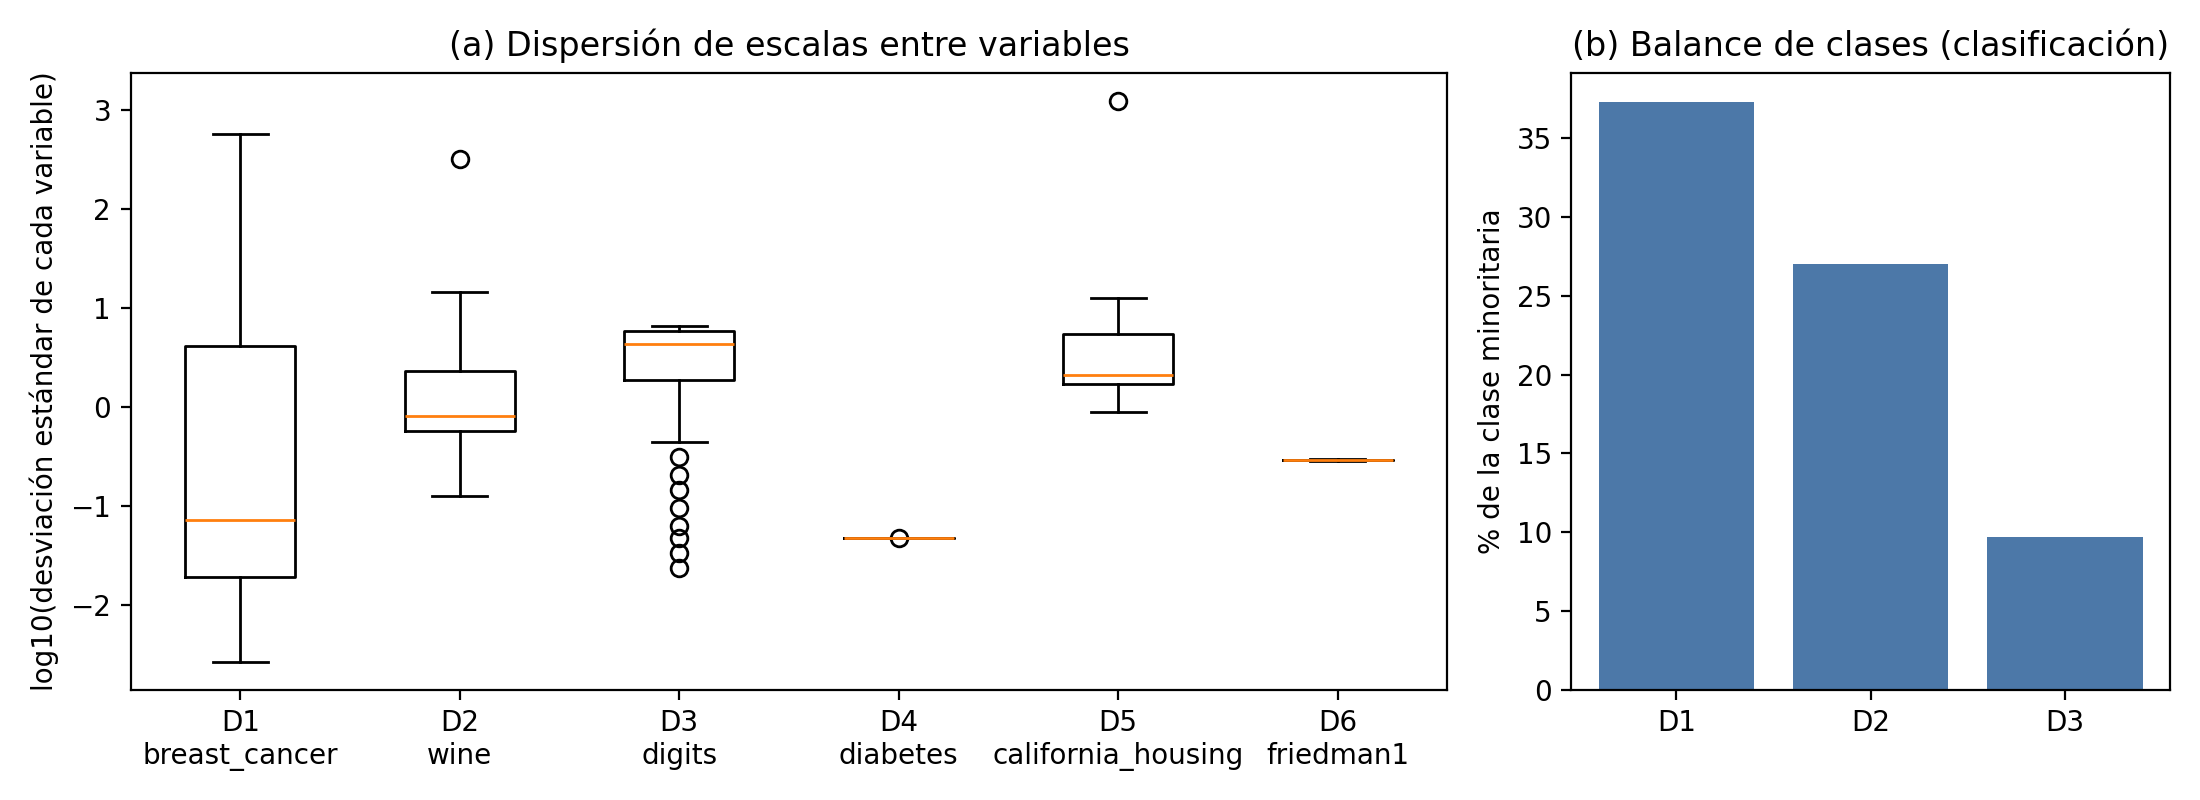
\includegraphics[width=0.82\textwidth]{fig_eda_datasets.png}
\caption{(a) Dispersión de escalas entre variables, en $\log_{10}$ de la desviación estándar. (b) Porcentaje de la clase minoritaria en los datasets de clasificación.}
\label{fig:eda}
\end{figure}

\textbf{Preparación trazable.} (i) \emph{Variante «completo»}: sin faltantes. (ii) \emph{Variante «con\_faltantes»}: se borra el 10\,\% de las celdas con semilla fija (media observada entre 9,8 y 10,1\,\%). (iii) A D1--D5 se les agregan 50 columnas de ruido gaussiano, porque la fuga por selección solo se manifiesta si hay variables inútiles entre las cuales elegir; D6 ya trae 45. Todo usa la semilla 42, y dos ejecuciones producen datos idénticos (verificado en las pruebas automáticas).

\textbf{Representatividad y limitaciones.} Son datasets clásicos, limpios, pequeños y tabulares; no representan datos reales ruidosos, de gran escala ni con estructura temporal o jerárquica, y los LLM probablemente los vieron durante su entrenamiento. Por la dispersión de escalas (Figura~\ref{fig:eda}a), el escalado debería afectar sobre todo a los modelos sensibles a la escala; por la asimetría de D5 (10,0) se esperan valores atípicos que desestabilicen a la red neuronal, y así ocurrió (sección~\ref{sec:desviaciones}). Con ROC-AUC cercana a 1 en D1--D3 hay un efecto techo que limita cuánto optimismo puede observarse en clasificación.

\section{Diseño experimental y arquitectura por fase}
\label{sec:diseno}
\label{sec:arquitectura}

Para cada combinación de 6 datasets $\times$ 4 familias $\times$ 4 tipos de fuga, un generador escribe un script con fuga (\texttt{leaky}) y otro idéntico sin ella (\texttt{clean}): \textbf{96 pares, 192 scripts}. Los modelos son \texttt{RandomForest}, \texttt{HistGradientBoosting}, \texttt{LogisticRegression} o \texttt{Ridge}, y \texttt{MLPClassifier} o \texttt{MLPRegressor}, todos de scikit-learn \parencite{pedregosa2011}. Como la verdad se conoce por construcción, no se necesitan anotadores.

Cada script se audita con \textbf{dos mecanismos independientes}. El primero analiza el árbol sintáctico (\texttt{ast}) con tres reglas: \emph{R-Split} (ajuste antes de \texttt{train\_test\_split}), \emph{R-CV} (ajuste fuera de un \texttt{Pipeline} cuyo resultado entra a la validación cruzada) y \emph{R-Test} (ajuste con una variable que parece de prueba). El segundo es un verificador en ejecución que cuenta con cuántas filas se ajusta cada transformador y declara fuga si coincide con el total del dataset. El detector híbrido declara fuga si cualquiera de los dos la ve.

Para evitar el sesgo de autopreferencia, el protocolo separa a los sujetos de estudio del sistema de medición (Tabla~\ref{tab:arquitectura}): ningún LLM participa en la auditoría ni en el cálculo de las métricas.

\begin{table}[!htbp]
\centering
\caption{Arquitectura por fase: quién genera y quién audita.}
\label{tab:arquitectura}
\begingroup\scriptsize\singlespacing
\begin{tabular}{@{}p{3.0cm} p{4.2cm} p{5.6cm} p{1.6cm}@{}}
\toprule
Componente & Rol & Implementación & ¿Usa LLM? \\
\midrule
Conjunto A (generador) & Sujetos de estudio: pipelines escritos por LLM & Mismo \emph{prompt} para todos; versión exacta y fecha registradas (Capstone~II) & Sí \\
Conjunto B (banco de control) & Verdad conocida por construcción & \arch{generate_controlled_pairs.py}: 96 pares con y sin fuga & No \\
Conjunto manual & Control de la circularidad & 13 scripts escritos a mano con estilos que el generador no produce & No \\
Motor auditor & Instrumento de medición & AST (tres reglas) y verificación en ejecución; salida idéntica en cada corrida & No \\
\bottomrule
\end{tabular}
\endgroup
\end{table}

\section{Hoja de ruta actualizada y desviaciones}
\label{sec:desviaciones}

\begin{table}[!htbp]
\centering
\caption{Hoja de ruta con hitos y entregables (estado a octubre de 2026).}
\label{tab:plan}
\begingroup\scriptsize\singlespacing
\begin{tabular}{@{}p{2.4cm} p{6.6cm} p{4.6cm} p{1.4cm}@{}}
\toprule
Periodo & Actividad & Hito o entregable verificable & Estado \\
\midrule
Capstone I & Reformulación del problema y la métrica; datasets; banco de 96 pares; auditor AST y de ejecución; refactorizador; \DOpt; Skills y plataforma web (prototipo) & Repositorio público reproducible con un comando; este informe & Hecho \\
Capstone II, sem. 1--4 & Generar pipelines con 6--8 LLM reales (24 tareas por modelo) y auditarlos; ejecutarlos en un contenedor aislado & Conjunto A versionado; tasa de fuga por modelo con IC95\,\% & Pendiente \\
Capstone II, sem. 5--8 & Mejorar el auditor (alias de importación, funciones auxiliares, \texttt{ColumnTransformer}); ampliar la evaluación independiente de 13 a $\geq 60$ scripts & Auditor v2 con recall independiente $\geq 0{,}80$ (umbral fijado antes de evaluar) & Pendiente \\
Capstone II, sem. 9--12 & Datasets con señal débil; \DOpt{} por tramo de señal/ruido; piloto de uso con 3--5 personas & Tabla de \DOpt{} condicionada; informe del piloto & Pendiente \\
Capstone II, sem. 13--16 & Redacción final y defensa & Documento final y presentación & Pendiente \\
\bottomrule
\end{tabular}
\endgroup
\end{table}

\textbf{Desviaciones respecto del plan original} (justificación completa en \arch{07_report/decision_log.md}):
\begin{itemize}
  \item \textbf{B1.} \texttt{california\_housing} se submuestrea a 3.000 filas: \texttt{KNNImputer} crece con $n^2$ y el banco de 192 scripts no sería ejecutable en un portátil.
  \item \textbf{B2.} El sobremuestreo (SMOTE) no se mide, porque no pertenece a scikit-learn; el cuarto tipo es «combinada».
  \item \textbf{C1.} En la primera corrida, los modelos lineal y MLP sin escalar daban diferencias negativas por inestabilidad numérica (hasta $-0{,}155$ en \texttt{wine}); se añadió un escalador interno idéntico en ambas versiones (corrida descartada en \arch{results/run1_discarded/}).
  \item \textbf{C2.} Un \texttt{MLPRegressor} divergió en un pliegue ($R^2=-21$ en \texttt{california\_housing}; promedio $-3{,}86$). Se definió, \textbf{después de ver el problema}, que un par es degenerado si algún pliegue tiene $R^2<-1$; se excluyó 1 par de 96 y se lista aparte.
\end{itemize}

% ========================================
% CAPÍTULO 4: PROTOCOLO DE VALIDACIÓN, LÍNEA BASE Y RESULTADOS PRELIMINARES  (criterio 4)
% ========================================

\chapter{VALIDACIÓN, LÍNEA BASE Y RESULTADOS PRELIMINARES}
\label{ch:validacion}

\section{Protocolo para evitar la fuga en la propia evaluación}

Se aplica al experimento lo que se audita: (i) validación cruzada de 5 pliegues (estratificada en clasificación) con semilla 42 y los \textbf{mismos pliegues} para \texttt{leaky} y \texttt{clean}; (ii) en la versión \texttt{clean} y en el código reparado, todo el preprocesamiento va dentro de un \texttt{Pipeline}, de modo que se ajusta solo con el entrenamiento de cada pliegue; (iii) el verificador en ejecución comprueba que, en \texttt{clean}, ningún transformador vea tantas filas como el total (el máximo observado es 80,3\,\%); (iv) las pruebas estadísticas usan como unidad el \textbf{par} (dataset $\times$ tipo de fuga) y no los pliegues, que no son independientes.

\section{Métricas y líneas base}

Las métricas se derivan de los criterios de éxito (Tabla~\ref{tab:exito}). \emph{Del auditor} (positivo = «hay fuga»): precisión, recall, F1 y valor predictivo negativo (VPN), porque el error más costoso es declarar limpio un script con fuga (falsa seguridad); el recall de la evaluación independiente se acompaña de un intervalo exacto de Clopper--Pearson \parencite{clopper1934}, adecuado para muestras pequeñas. \emph{Del daño}: \DOpt{} en ROC-AUC (clasificación, insensible al umbral y al desbalance) y $R^2$ (regresión, comparable entre datasets), con F1 macro y RMSE como secundarias; la media de \DOpt{} por familia se informa con un intervalo bootstrap percentil del 95\,\% \parencite{efron1993}.

Se definen tres líneas base, cada una como punto de comparación de una afirmación distinta:
\begin{itemize}
  \item \textbf{Del daño:} el pipeline \texttt{clean}. Es el desempeño que se habría reportado sin el error, por lo que \DOpt{} mide exactamente el exceso atribuible a la fuga.
  \item \textbf{Del detector híbrido:} cada componente por separado (solo AST y solo ejecución). Justifica que combinar ambos aporte algo.
  \item \textbf{Externa:} una regla trivial (\arch{baseline_simple_rule.py}) que declara fuga si el script ajusta un transformador con \texttt{.fit} y no usa ningún \texttt{Pipeline}, ignorando comentarios e importaciones. Representa lo que haría un revisor apurado con una búsqueda de texto; si el auditor no la supera, su complejidad no se justifica. La escribió el autor y no es un \emph{linter} de terceros; la comparación con un LLM juez queda para Capstone~II.
\end{itemize}

\section{Resultados: eficacia del auditor}
\label{sec:eficacia}

\begin{table}[!htbp]
\centering
\caption{Banco de control: 192 scripts con verdad conocida.}
\label{tab:banco}
\begingroup\footnotesize\singlespacing
\begin{tabular}{@{}l r r r r r r r@{}}
\toprule
Detector & TP & TN & FP & FN & Precisión & Recall & VPN \\
\midrule
AST (estático) & 96 & 96 & 0 & 0 & 1,00 & 1,00 & 1,00 \\
Ejecución & 96 & 96 & 0 & 0 & 1,00 & 1,00 & 1,00 \\
Híbrido & 96 & 96 & 0 & 0 & 1,00 & 1,00 & 1,00 \\
\bottomrule
\end{tabular}
\endgroup
\end{table}
\donde{TP, TN, FP, FN: verdaderos positivos, verdaderos negativos, falsos positivos y falsos negativos; $\mathrm{Precisión}=TP/(TP+FP)$; $\mathrm{Recall}=TP/(TP+FN)$; $\mathrm{VPN}=TN/(TN+FN)$.}

\textbf{Este 100\,\% no prueba que el auditor generalice}: el banco lo produce un generador escrito por el mismo autor que el auditor (evaluación circular), con patrones que este conoce. Por eso se añadió una \textbf{evaluación independiente} con 13 scripts escritos a mano (9 con fuga y 4 limpios), con estilos que el generador no produce: \texttt{make\_pipeline}, DataFrames, funciones auxiliares, alias de importación, variables \texttt{X\_te}, y \texttt{fit} y \texttt{transform} por separado.

\begin{table}[!htbp]
\centering
\caption{Evaluación independiente ($n=13$) y línea base externa (regla simple).}
\label{tab:indep}
\label{tab:base}
\begingroup\footnotesize\singlespacing
\begin{tabular}{@{}l l r r r r r c@{}}
\toprule
Conjunto & Detector & TP & FP & FN & Precisión & VPN & Recall [IC95\,\%] \\
\midrule
Independiente (13) & Regla simple & 8 & 1 & 1 & 0,89 & 0,75 & 0,89 [0,52; 1,00] \\
 & AST & 8 & 0 & 1 & 1,00 & 0,80 & 0,89 [0,52; 1,00] \\
 & Ejecución & 7 & 0 & 2 & 1,00 & 0,67 & 0,78 [0,40; 0,97] \\
 & Híbrido & 9 & 0 & 0 & 1,00 & 1,00 & 1,00 [0,66; 1,00] \\
\midrule
Banco (192) & Regla simple & 72 & 0 & 24 & 1,00 & 0,80 & 0,75 [0,65; 0,83] \\
 & Híbrido & 96 & 0 & 0 & 1,00 & 1,00 & 1,00 \\
\bottomrule
\end{tabular}
\endgroup
\end{table}
\nota{IC95\,\%: intervalo exacto de Clopper--Pearson para el recall. Conjunto independiente: 9 scripts con fuga y 4 limpios.}

La regla simple rinde sorprendentemente bien en los casos manuales (recall 0,89, igual que el AST), pero con un falso positivo (declara fuga en el script que escala \emph{después} de dividir) y deja pasar el alias de importación; en el banco pierde 24 de 96 fugas. El AST falla con el alias (\texttt{StandardScaler as SS}); la ejecución falla con ajustes que no usan todas las filas (el escalador re-ajustado con las filas de prueba y el ajustado con el 70\,\% de entrenamiento antes de la validación cruzada). Fallan en casos distintos, lo que respalda el diseño híbrido. Pero los intervalos se solapan ampliamente: con $n=9$ casos con fuga, el límite inferior del recall híbrido es 0,66, y la ventaja sobre la línea base es un margen que Capstone~II debe confirmar, no una mejora demostrada. La reparación automática resolvió 4 de los 9 scripts con fuga; en los otros 5 declaró «requiere revisión manual» y no tocó el código.

\section{Resultados preliminares: Sesgo de Optimismo}
\label{sec:dopt}

\begin{figure}[!htbp]
\centering
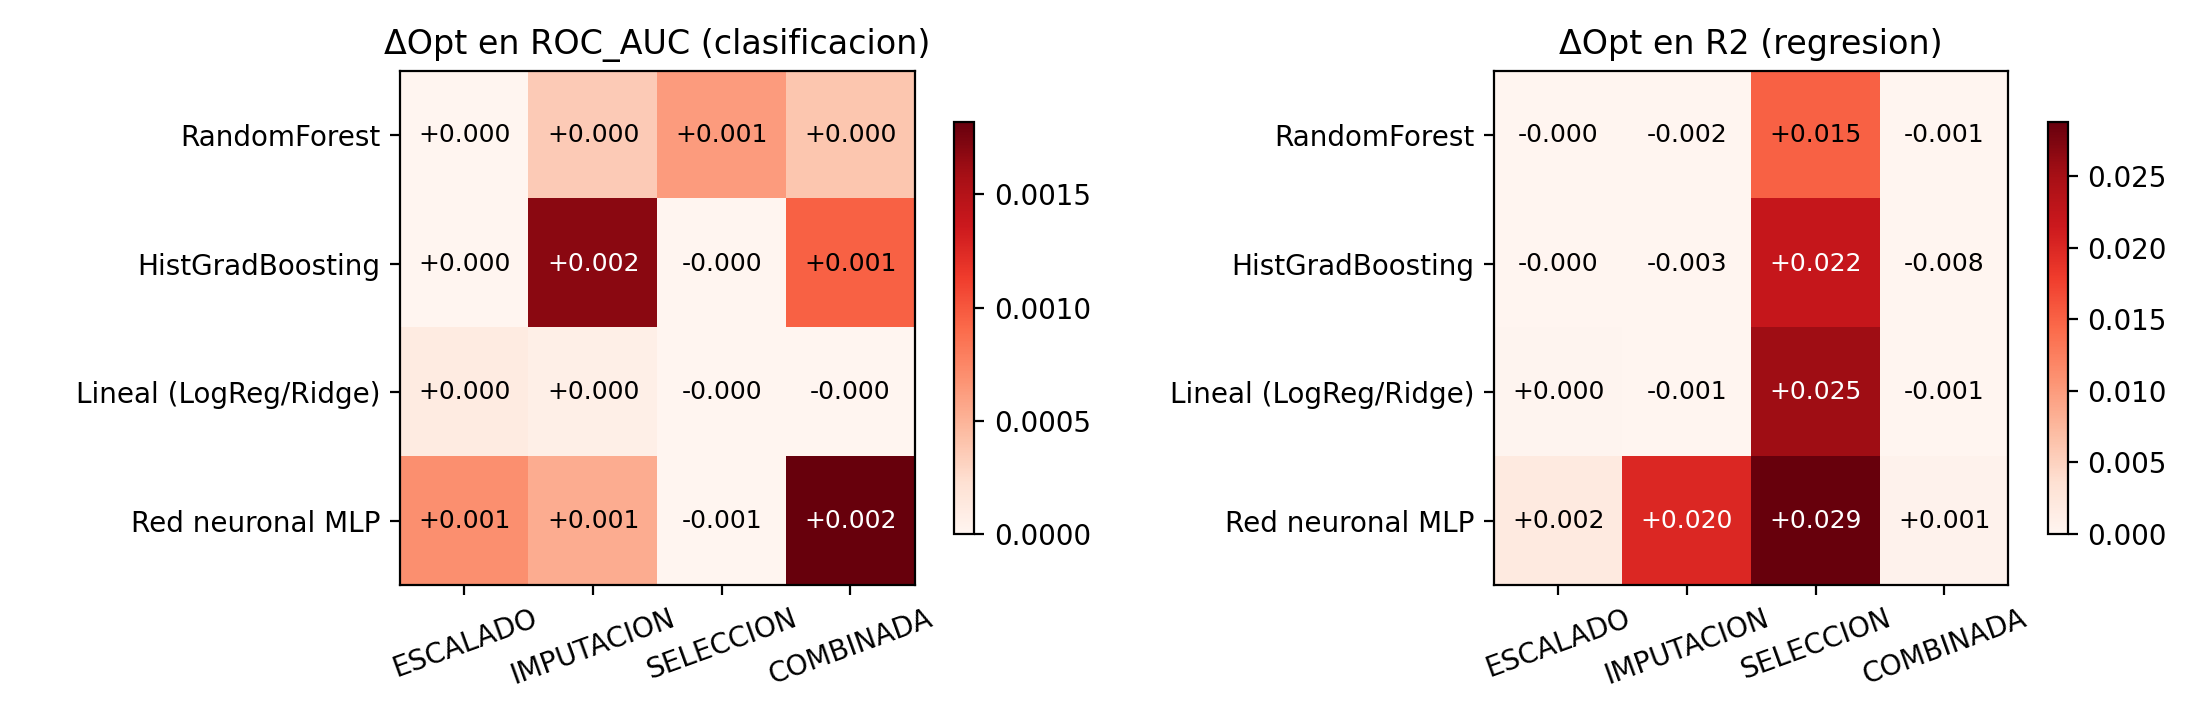
\includegraphics[width=0.88\textwidth]{fig_delta_opt_heatmap.png}
\caption{\DOpt{} medio por familia y tipo de fuga (ROC-AUC en clasificación, $R^2$ en regresión). El par degenerado (D5, MLP, combinada) está excluido.}
\label{fig:heatmap}
\end{figure}

\begin{table}[!htbp]
\centering
\caption{\DOpt{} medio, promedio sobre los datasets.}
\label{tab:dopt}
\begingroup\footnotesize\singlespacing
\begin{tabular}{@{}l l r r r r@{}}
\toprule
Tarea & Familia & Escalado & Imputación & Selección & Combinada \\
\midrule
Clasificación (AUC) & RandomForest & 0,0000 & 0,0004 & 0,0006 & 0,0004 \\
 & Gradient Boosting & 0,0000 & 0,0017 & $-0{,}0001$ & 0,0010 \\
 & Lineal & 0,0001 & 0,0001 & $-0{,}0001$ & 0,0000 \\
 & MLP & 0,0007 & 0,0005 & $-0{,}0009$ & 0,0018 \\
\midrule
Regresión ($R^2$) & RandomForest & $-0{,}0001$ & $-0{,}0024$ & 0,0150 & $-0{,}0014$ \\
 & Gradient Boosting & 0,0000 & $-0{,}0033$ & 0,0220 & $-0{,}0082$ \\
 & Lineal & 0,0001 & $-0{,}0008$ & 0,0255 & $-0{,}0007$ \\
 & MLP & 0,0019 & 0,0200 & 0,0288 & 0,0006$^{*}$ \\
\bottomrule
\end{tabular}
\endgroup
\end{table}
\nota{$^{*}$Media de 2 datasets (se excluyó el par degenerado).}

Se observan tres hechos. \textbf{(1) En clasificación, \DOpt{} es prácticamente nulo}: en 48 pares va de $-0{,}0027$ a $+0{,}0034$, con un AUC limpio mediano de 0,991 (efecto techo). \textbf{(2) En regresión aparece optimismo, concentrado en la selección con \texttt{california\_housing}}: $R^2$ de 0,690 (sin fuga) frente a 0,731 (con fuga) en RandomForest, y de 0,615 frente a 0,689 en MLP; en los 47 pares el rango es de $-0{,}023$ a $+0{,}074$. \textbf{(3) Escalado y árboles:} en RandomForest y HistGradientBoosting, en los 6 datasets, el máximo $|\DOpt|$ por escalado es 0,0002, como predice la teoría: una transformación afín creciente no cambia la estructura de un árbol.

\begin{table}[!htbp]
\centering
\caption{Pruebas por familia en regresión (fugas simples, $n=9$ pares).}
\label{tab:tests}
\begingroup\footnotesize\singlespacing
\begin{tabular}{@{}l r c r r r@{}}
\toprule
Familia & \DOpt{} medio & IC95\,\% bootstrap & $d$ de Cohen & $p$ Wilcoxon & $p$ Holm \\
\midrule
RandomForest & 0,0042 & [$-0{,}0023$; 0,0142] & 0,29 & 0,320 & 1,000 \\
Gradient Boosting & 0,0062 & [$-0{,}0021$; 0,0199] & 0,32 & 0,371 & 1,000 \\
Lineal (Ridge) & 0,0083 & [$-0{,}0015$; 0,0250] & 0,34 & 0,285 & 1,000 \\
MLP & 0,0169 & [0,0027; 0,0346] & 0,65 & \textbf{0,037} & 0,297 \\
\bottomrule
\end{tabular}
\endgroup
\end{table}
\nota{Hipótesis alternativa: $\DOpt>0$ (Wilcoxon unilateral). IC95\,\%: bootstrap percentil de la media con 10.000 remuestreos (semilla 42). $p$ Holm: ajuste de Holm sobre las 8 pruebas (2 tareas $\times$ 4 familias). Se usan las fugas simples porque la combinada repite esos mecanismos.}

En clasificación, el $p$ de Wilcoxon de todas las familias es $\geq 0{,}148$ y todos los intervalos incluyen el cero. En regresión, la MLP es la única familia cuyo intervalo excluye el cero y cuyo $p$ sin corregir es menor que 0,05, pero tras el ajuste de Holm \parencite{holm1979} su $p$ sube a 0,297. La prueba de Friedman entre familias da $p=0{,}84$ en clasificación y $p=0{,}041$ en regresión (rangos medios, donde 1 indica el mayor optimismo: RandomForest 3,39; Gradient Boosting 2,72; Lineal 2,11; MLP 1,78), que con la corrección de Bonferroni para dos pruebas pasa a 0,082. Por eso las diferencias entre familias se reportan como \textbf{exploratorias} \parencite{demsar2006}.

\section{Control positivo: cuándo la selección con fuga sí daña}
\label{sec:control}

Para comprobar que \DOpt{} detecta la fuga cuando esta importa, se repitió solo la selección con 0, 50, 200 y 1000 columnas de ruido, en dos escenarios: \emph{real} (etiquetas verdaderas) y \emph{señal nula} (etiquetas permutadas al azar, de modo que la verdad es AUC $=0{,}5$ y $R^2\leq 0$).

\begin{figure}[!htbp]
\centering
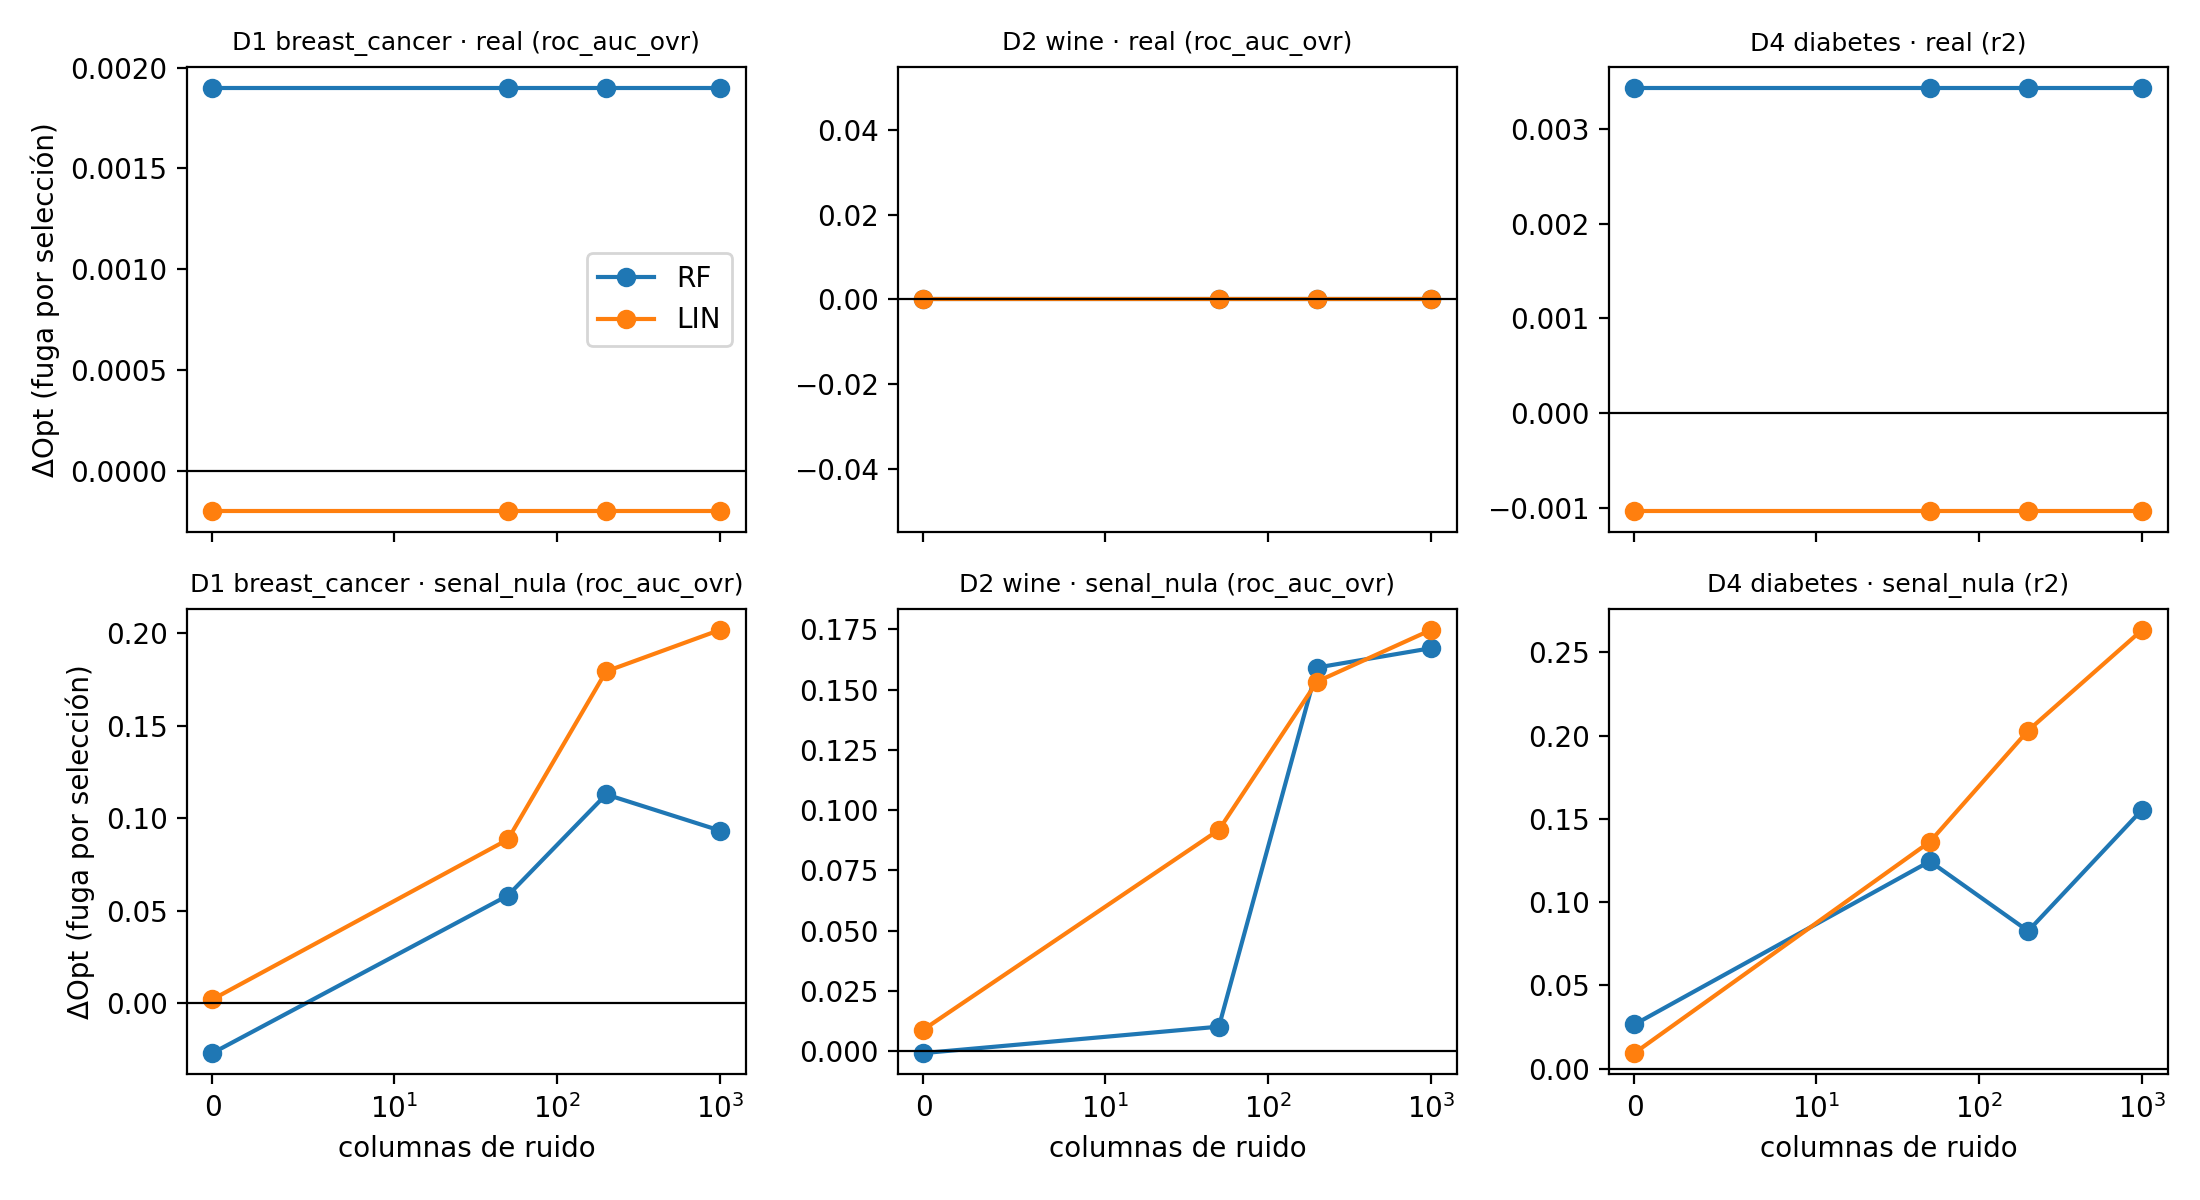
\includegraphics[width=0.95\textwidth]{fig_noise_sensitivity.png}
\caption{\DOpt{} de la selección con fuga según el número de columnas de ruido. Fila superior: etiquetas reales. Fila inferior: señal nula (control positivo).}
\label{fig:ruido}
\end{figure}

Con etiquetas reales, \DOpt{} \textbf{no cambia} con el ruido (por ejemplo, \texttt{breast\_cancer} con RandomForest: 0,0019 en los cuatro niveles), porque con al menos 8 variables muy informativas el selector nunca elige columnas de ruido. Con señal nula crece con el ruido hasta \textbf{$+0{,}20$ de AUC} (\texttt{breast\_cancer}, lineal, 1000 columnas) y \textbf{$+0{,}26$ de $R^2$} (\texttt{diabetes}, lineal): el selector «encuentra» columnas de ruido que, por azar, parecen predecir.

% ========================================
% CAPÍTULO 5: INTERPRETACIÓN Y JUICIO CRÍTICO  (criterio 5)
% ========================================

\chapter{INTERPRETACIÓN Y JUICIO CRÍTICO}
\label{ch:interpretacion}

\textbf{Qué indican los resultados.} (a) El auditor reconoce con fiabilidad los patrones para los que fue diseñado, pero el 100\,\% del banco \textbf{no} es evidencia de generalización: la prueba independiente baja el recall del AST a 0,89 y el del verificador a 0,78, y cada uno falla donde el otro acierta. La conclusión sostenible es que \textbf{la combinación es más robusta que cada parte}, no que el auditor sea casi perfecto. (b) La fuga de preprocesamiento y selección tuvo un efecto pequeño en los datasets elegidos, no porque sea inocua sino porque estos datos son «fáciles»: señal fuerte y AUC en el techo. El control positivo muestra que, cuando la señal es débil frente al ruido, el mismo mecanismo infla la métrica hasta 0,20--0,26; la gravedad depende de la relación entre señal y ruido y no es una propiedad fija de cada tipo de fuga ni de cada familia de modelos. (c) De las dos hipótesis de la reformulación, la del escalado en árboles se confirma con claridad; la de que la red neuronal es la más vulnerable tiene respaldo débil: se observa en regresión (\DOpt{} medio 0,017; $d=0{,}65$) pero no en clasificación, y no resiste la corrección por multiplicidad.

\textbf{Implicaciones para la factibilidad.} El proyecto es factible como instrumento (detectar, reparar y medir) y se puede defender con lo hecho. Es menos sólido como afirmación empírica sobre «qué modelos sufren más», porque hay solo 3 datasets por tarea y 9 pares por familia. Por eso el objetivo OE3 se reformula para Capstone~II: estimar \DOpt{} \textbf{condicionado a la razón señal/ruido}, y no como un número único por familia.

\textbf{Limitaciones y amenazas a la validez.} \emph{Datos:} seis datasets clásicos que los LLM probablemente conocen, un submuestreo de \texttt{california\_housing} y un efecto techo en clasificación. \emph{Método:} el generador y el auditor tienen el mismo autor (circularidad), la prueba independiente tiene 13 casos, la exclusión de un par degenerado fue posterior a ver el problema y los valores $p$ no están corregidos. \emph{Generalización:} los resultados valen para pipelines sintéticos de scikit-learn; \textbf{aún no se sabe qué tan frecuente es la fuga en código escrito por LLM reales}, que es la pregunta motivadora del proyecto, ni cómo se comporta el auditor ante su variedad de estilos.

\textbf{Riesgos para Capstone~II y ajustes propuestos.} La Tabla~\ref{tab:riesgos} los resume junto con la evidencia que los respalda.

\begin{table}[!htbp]
\centering
\caption{Riesgos observados, evidencia y ajustes para Capstone~II.}
\label{tab:riesgos}
\begingroup\footnotesize\singlespacing
\begin{tabular}{@{}p{4.4cm} p{4.0cm} p{6.6cm}@{}}
\toprule
Riesgo & Evidencia & Ajuste \\
\midrule
El código de LLM reales es más variado que las plantillas y el recall caerá & AST 0,89 y ejecución 0,78 en código escrito a mano & Ampliar la prueba independiente a $\geq 60$ scripts y, con los LLM reales, etiquetar una muestra a mano con revisión cruzada \\
Alias, funciones auxiliares y reparaciones manuales (solo 4/9 reparados) & Un caso con alias; cuatro casos sin reparación automática & Resolver alias de importación; ampliar el refactorizador a \texttt{ColumnTransformer} y funciones \\
Efecto techo y pocos datasets & AUC mediano 0,991; $|\DOpt|\leq 0{,}0034$ en clasificación & Incorporar datasets de señal débil o con muchas más variables que filas; informar \DOpt{} por tramo de señal/ruido \\
Ejecutar código de LLM es riesgoso & --- & Ejecutar solo en contenedor sin red ni credenciales; la plataforma web seguirá sin ejecutar código \\
Costo y términos de servicio de las APIs & Script de generación sin probar & Medir tokens con 2 modelos antes de escalar; revisar términos de publicación de salidas \\
\bottomrule
\end{tabular}
\endgroup
\end{table}

% ========================================
% CAPÍTULO 6: APLICABILIDAD Y USO RESPONSABLE  (criterio 6)
% ========================================

\chapter{APLICABILIDAD Y USO RESPONSABLE}
\label{ch:aplicabilidad}

\section{Contexto de uso}

Los usuarios previstos son (1) analistas y estudiantes de ciencia de datos que reciben pipelines de un asistente de IA y (2) equipos que quieren una revisión automática antes de integrar código a un repositorio. La decisión que informa el auditor es: \emph{aceptar, corregir o derivar a revisión humana} un pipeline. Los tres productos comparten el mismo núcleo (\arch{03_auditor/}), de modo que un script recibe el mismo veredicto por cualquier vía.

\section{Propuesta de implementación}

\textbf{Skills para agentes} (\arch{05_skills/}). \texttt{audit-ml-leakage} audita y repara scripts existentes; \texttt{create-\allowbreak leakage-\allowbreak free-\allowbreak pipeline} impone reglas al crear código (todo preprocesamiento dentro de un \texttt{Pipeline}, prueba final apartada, semillas fijas) y exige autoverificarse con el auditor antes de entregar. Cada Skill es una carpeta autocontenida que se copia al directorio de Skills del agente. La herramienta de línea de comandos devuelve el código de salida 0 (limpio) o 1 (fuga), por lo que también puede bloquear una integración continua.

\textbf{Plataforma web en Streamlit} (\arch{06_web_app/}), pensada para quien no usa agentes de programación. Su diseño separa tres capas: la interfaz (\arch{app.py}), que solo dibuja pantallas; la lógica (\arch{app_logic.py}), que valida la entrada, invoca al auditor, resalta líneas y calcula diferencias, y que se prueba sin navegador; y el núcleo auditor compartido. El flujo de uso tiene cuatro pestañas: (1) \emph{auditar y reparar}: el usuario pega o sube un \texttt{.py}, ve en rojo las líneas con fuga y la regla que las explica, y puede descargar la versión corregida junto con sus diferencias; (2) \emph{cuánto infla la fuga}: consulta \DOpt{} para cualquier combinación de dataset, familia y tipo de fuga del experimento; (3) \emph{resultados del experimento}: eficacia del auditor y pruebas por familia; y (4) \emph{guía}: qué es la fuga, ejemplos y limitaciones.

\emph{Requisitos:} Python (probado con la versión 3.13), scikit-learn y Streamlit, con versiones fijas en \arch{requirements.txt}. \emph{Condiciones de uso:} scripts tabulares con scikit-learn; los notebooks se exportan a \texttt{.py}. \emph{Verificación hecha:} pruebas automáticas que cubren el auditor, la reparación, las Skills y el arranque de la plataforma web. \emph{Monitoreo:} registrar los falsos negativos que reporten los usuarios y convertirlos en casos de prueba. \textbf{Aún no se ha hecho una prueba de uso con personas}; el producto es un prototipo y esa prueba queda para Capstone~II.

\section{Riesgos éticos y medidas}

La Tabla~\ref{tab:etica} identifica los riesgos propios de este caso y la medida concreta que los aborda, junto con la forma de comprobar que la medida existe.

\begin{table}[!htbp]
\centering
\caption{Riesgos de uso responsable, medidas y verificación.}
\label{tab:etica}
\begingroup\scriptsize\singlespacing
\begin{tabular}{@{}p{2.6cm} p{4.4cm} p{4.6cm} p{3.2cm}@{}}
\toprule
Riesgo & Por qué aplica a este proyecto & Medida concreta & Verificación \\
\midrule
Falsa seguridad & «0 fugas» puede leerse como «sin fuga», pero no se ven fugas temporales, de dominio, por duplicados ni código dinámico & La web, la línea de comandos y las Skills muestran que el resultado significa «sin evidencia de las reglas R-Split, R-CV y R-Test» & Texto visible en la pestaña 1 y en ambos \arch{SKILL.md} \\
Ejecución de código no confiable & El código de LLM o de usuarios puede ser malicioso & La web solo lee el código (AST) y nunca lo ejecuta; rechaza entradas de más de 200.000 caracteres y escapa el HTML; el código de LLM se ejecutará solo en un contenedor sin red ni credenciales & Pruebas automáticas de escape de HTML y de límite de tamaño \\
Datos sensibles & \texttt{breast\_cancer} y \texttt{diabetes} son datos clínicos & Se usan solo conjuntos públicos y anonimizados de scikit-learn, sin fines clínicos; la web no guarda el código que se le entrega & Carga desde \texttt{sklearn.datasets}; sin almacenamiento en la aplicación \\
Sesgo del instrumento & El auditor se probó con estilos de un solo autor & Evaluación independiente separada del banco; se informan los fallos conocidos (alias de importación) & Tabla~\ref{tab:indep}; casos 05 y 09 \\
Términos de servicio & Las salidas de las APIs de LLM pueden tener restricciones de publicación & Revisar los términos de cada proveedor antes de publicar el Conjunto A & Registro en \arch{decision_log.md} \\
\bottomrule
\end{tabular}
\endgroup
\end{table}
\nota{No se evalúa la equidad de los modelos entrenados porque no es el objeto del estudio; se declara como límite.}

\textbf{Declaración de uso de inteligencia artificial.} El problema, las ideas, el diseño del estudio y el borrador del informe son del autor. Se utilizó un asistente de programación basado en IA como apoyo para implementar y comentar el código, organizar el repositorio y editar la redacción a partir de ese borrador. Las cifras provienen de la ejecución del código y se contrastaron con los archivos de resultados; el autor es responsable del contenido y de su defensa.

% ========================================
% CAPÍTULO 7: CONCLUSIONES
% ========================================

\chapter{CONCLUSIONES}
\label{ch:conclusiones}

La pregunta de investigación tiene, con la evidencia de Capstone~I, una respuesta afirmativa pero acotada. \textbf{Detectar} es posible: el auditor determinista reconoce la fuga de preprocesamiento y selección en scripts de scikit-learn, y en una prueba independiente pequeña el diseño híbrido detectó los 9 casos con fuga, aunque ninguno de sus dos componentes lo logró por sí solo (OE2). \textbf{Reparar sin cambiar el modelo} es posible en los patrones habituales, pero no en general: 96 de 96 en el banco y 4 de 9 en código escrito a mano (OE4). \textbf{Cuantificar} es posible con \DOpt, un indicador pareado que separa la fuga del sobreajuste; su magnitud no es una propiedad fija de cada familia de modelos, sino que depende de la relación entre señal y ruido: casi nula con datos de señal fuerte y de hasta 0,20 de AUC con señal nula (OE3). Los productos, dos Skills y una plataforma web, están operativos como prototipo (OE4).

Lo que falta, y es lo que da sentido al proyecto, es medir la fuga en código escrito por LLM reales. Para Capstone~II se fijan de antemano los umbrales, se amplía la evaluación independiente y se reformula OE3 en términos de señal y ruido. Todas las cifras de este informe y el código que las produce están en el repositorio y se regeneran con un solo comando.


\chapter*{REFERENCIAS}
\addcontentsline{toc}{chapter}{REFERENCIAS}

\printbibliography[heading=none]

\newpage
\thispagestyle{empty}
\begin{center}
    \vspace*{8cm}
    {\Huge\textbf{ANEXOS}}
    \vfill
\end{center}
\newpage

% ========================================
% ANEXOS (no cuentan en la extensión del informe)
% ========================================

\anexo{REPRODUCIBILIDAD Y REPOSITORIO}
\label{an:repro}

\textbf{Repositorio:} \url{https://github.com/witman92/ml-leakage-auditor-capstone}.

Todas las tablas y figuras de este informe se generan en \arch{04_experiments/results/} y se reproducen con:

\begin{footnotesize}
\begin{verbatim}
pip install -r requirements.txt
python 04_experiments/leakage_demo.py   # ejemplo visual (Figura 1.2)
python run_all.py                       # fases 0-5, estadistica, figuras y pruebas
python run_all.py --rapido              # verificacion rapida (2 datasets x 2 familias)
streamlit run 06_web_app/app.py         # plataforma web
\end{verbatim}
\end{footnotesize}

\textbf{Estructura del repositorio.} Cada carpeta numerada corresponde a una fase del protocolo (Tabla~\ref{tab:etapas}):

\begin{footnotesize}
\begin{verbatim}
ml-leakage-auditor-capstone/
|-- run_all.py                  # reproduce todo con un comando
|-- requirements.txt            # versiones fijas (Python 3.13)
|-- 01_data/                    # Fase 0: carga de los 6 datasets de scikit-learn
|-- 02_pipelines/               # Fase 1: banco de 96 pares (controlled_pairs/),
|                               #   reparados (repaired_pairs/) y Conjunto A (llm_generated/)
|-- 03_auditor/                 # Fase 2: AST, verificador en ejecucion, refactorizador, CLI
|-- 04_experiments/             # Fases 3-4: benchmark, EDA, estadistica, demo, linea base
|   `-- results/                #   tablas (.csv), figuras (.png), manifiesto de ejecucion
|-- 05_skills/                  # Fase 5: dos Agent Skills autocontenidas
|-- 06_web_app/                 # Fase 5: plataforma web en Streamlit
|-- 07_report/                  # informe LaTeX, registro de decisiones, checklist
`-- 08_tests/                   # pruebas automaticas y 13 casos escritos a mano
\end{verbatim}
\end{footnotesize}

Cada script está organizado en bloques numerados (\texttt{\# \%\% PASO n}) que se pueden ejecutar uno a uno en VS Code o en Colab, y cada bloque explica de dónde vienen los datos, qué hace la función, qué métrica o gráfico produce y cómo interpretarlo. \arch{run_benchmark.py} escribe además \arch{run_manifest.json} con las versiones de las librerías y la semilla, y ordena todas las tablas de salida, de modo que dos ejecuciones producen archivos idénticos. La carpeta se abre en VS Code con \arch{capstone.code-workspace}, que trae una tarea por fase. Las decisiones y desviaciones están en \arch{07_report/decision_log.md}.


\end{document}
